\documentclass[]{article}

\usepackage{graphicx}
\usepackage{url}
\usepackage{hyperref}

%opening
\title{Bachelor Thesis: Incorporating affective states of players in video games}
\date{September 19, 2011}

\begin{document}

\maketitle

\begin{description}
	\centering
	\item[] \textbf{Supervisor}: Dr. Muharram Mansoorizadeh
\end{description}

\begin{abstract}

Video games are very popular, these days. They use different ways to interact with users. Keyboards, mouse, Joysticks, and recently camera are among the popular interaction devices. While technology involved in game industry develops new interactive devices to get user's interactions that capture lots of player's inputs, the games just use player's voluntary interactions. However, spontaneous behaviors of players are of much value in playing games, the players do not use involuntary interactions. Among several available representations for affects, two-dimensional continuous Activation/Evaluation(Valence) space has been adopted. We can determine the player's preferences in the environment by comparing his or her playing to the player's valence and activity in real-time. These information can be used to modify the game rules and environment to make it more attractive for players and create a unique experience during each gameplay session.\newline


Implemented using \textbf{C++}, and \textbf{DirectX 10}.\newline

More information can be found on:\

\href{https://mmostajab.com/bachelor-thesis/}{https://mmostajab.com/bachelor-thesis/}

\end{abstract}


\begin{figure}[ht!]
	\centering
	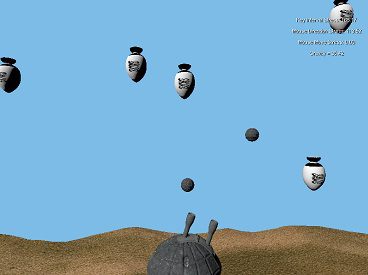
\includegraphics[width=0.4\linewidth]{stressbasedgame.jpg}
	\caption{A screenshot of the developed affective game for my bachelor thesis.}
	\label{fig:boat1}
\end{figure}

\end{document}
